\section{流形上的函数空间}
\label{sec:mcalc-function-spaces}

上一节的弱梯度与弱形式需要一个函数类：函数本身可积到什么程度，弱导数可积到什么程度。欧氏区域上，这由$L^p$与Sobolev空间回答（第~\ref{chap:function-normed-spaces}章与第~\ref{chap:sobolev-spaces}章）。流形上没有全局坐标，但紧流形可以用有限张坐标图覆盖，每张图里都可以借用欧氏的结果。

本节说明怎样把这些空间搬到紧流形上，哪些性质能搬，搬的时候要核对什么。非紧流形放在最后讨论。

\paragraph{$L^p$空间}
第~\ref{sec:mcalc-function-integration}小节已经把黎曼体积做成$M$上的测度$\operatorname{vol}_g$。对$1\leq p<\infty$，定义
\begin{equation}
\lVert u\rVert_{L^p(M,g)}=\Bigl(\int_M\lvert u\rvert^p\,\mathrm dV_g\Bigr)^{1/p},
\label{eq:mcalc-lp-norm}
\end{equation}
$L^p(M,g)$是使其有限的可测函数（几乎处处相等者视为同一元素）组成的空间；$p=\infty$时取本性上确界。这是一般测度空间上的$L^p$空间的特例，所以第~\ref{chap:function-normed-spaces}章的结论直接适用：它是Banach空间，$p=2$时是Hilbert空间。可测向量场$Y$属于$L^p$，指函数$\lVert Y\rVert_g$属于$L^p(M,g)$，这样的向量场同样构成Banach空间。

\begin{theorem}[紧流形上$L^p$与度量的选择无关]
\label{thm:mcalc-lp-metric-independence}
设$M$是紧流形，$g$与$g'$是$M$上的两个黎曼度量，$1\leq p<\infty$。则存在常数$0<c\leq C$，使对所有可测函数$u$，
\begin{equation}
c\,\lVert u\rVert_{L^p(M,g)}\leq\lVert u\rVert_{L^p(M,g')}\leq C\,\lVert u\rVert_{L^p(M,g)}.
\label{eq:mcalc-lp-equivalence}
\end{equation}
因此$L^p(M,g)$与$L^p(M,g')$是同一个函数集合，范数等价。
\end{theorem}

\begin{proof}
在任一坐标图中令$\kappa=\sqrt{\det\bm G'}/\sqrt{\det\bm G}$。由式~\eqref{eq:mcalc-density-change}，换图时分子分母都乘以$\lvert\det\bm A\rvert$，所以$\kappa$是$M$上与坐标无关的函数，并且连续、处处为正，满足$\mathrm dV_{g'}=\kappa\,\mathrm dV_g$。

紧集上的正连续函数有正的最小值$m$和有限的最大值$m'$，于是
\[
m\int\lvert u\rvert^p\,\mathrm dV_g\leq\int\lvert u\rvert^p\,\mathrm dV_{g'}\leq m'\int\lvert u\rvert^p\,\mathrm dV_g .
\]
开$p$次方即得，$c=m^{1/p}$，$C=m'^{1/p}$。
\end{proof}

所以在紧流形上，“$u$属于$L^p$”是一个不依赖度量的性质，度量只影响范数的具体数值。球面的半径变化是这个定理的最简单情形：半径$a$的球面上$\mathrm dV=a^2\,\mathrm dV_{S^2}$，常数$c=C=a^{2/p}$。

\paragraph{Sobolev空间的内在定义}
有了第~\ref{sec:mcalc-integration-by-parts}节的弱梯度，一阶Sobolev空间可以不借坐标定义。设$M$是紧流形（暂设无边界），$1\leq p<\infty$。若$u\in L^p(M,g)$存在弱梯度$Y$且$Y$属于$L^p$，称$u\in W^{1,p}(M)$，记$\operatorname{grad}u=Y$，并取范数
\begin{equation}
\lVert u\rVert_{W^{1,p}}=\Bigl(\lVert u\rVert_{L^p}^p+\bigl\lVert\,\lVert\operatorname{grad}u\rVert_g\bigr\rVert_{L^p}^p\Bigr)^{1/p}.
\label{eq:mcalc-sobolev-norm}
\end{equation}

弱梯度若存在则几乎处处唯一：两个弱梯度之差$Z$满足$\int g(Z,X)\,\mathrm dV_g=0$对所有光滑$X$成立，在每张坐标图中用光滑向量场逼近$Z$的截断，即得$Z=0$几乎处处，这与第~\ref{chap:smoothing-weak-derivatives}章中弱导数唯一性的论证相同。

前面$S^1$上的$u=\lvert\theta\rvert$就在这个空间里。它的弱梯度是$\operatorname{sgn}(\theta)\,\partial_\theta$，其度量长度恒为$1$。对比圆周上的光滑函数$u_0=1+\tfrac12\cos\theta$，它的$W^{1,2}$范数可以直接计算：
\[
\lVert u_0\rVert_{L^2}^2=\int_0^{2\pi}\bigl(1+\tfrac12\cos\theta\bigr)^2\,\mathrm d\theta=\frac94\pi ,\qquad
\lVert u_0'\rVert_{L^2}^2=\frac\pi4 .
\]
两者相加，$\lVert u_0\rVert_{W^{1,2}}^2=\tfrac52\pi$。这里用的是$S^1$的标准度量；下面的定理说明这个空间在选取度量之后的性质。

\begin{theorem}[$W^{1,p}(M)$的完备性]
\label{thm:mcalc-sobolev-complete}
在紧黎曼流形上，$W^{1,p}(M)$是Banach空间。
\end{theorem}

\begin{proof}
设$(u_m)$是$W^{1,p}$中的Cauchy列，则$(u_m)$与$(\operatorname{grad}u_m)$分别是$L^p$函数与$L^p$向量场中的Cauchy列。由$L^p$的完备性，$u_m\to u$，$\operatorname{grad}u_m\to Y$。

对任一光滑向量场$X$，$\operatorname{div}X$与$\lVert X\rVert_g$在紧集$M$上有界，由Hölder不等式，式~\eqref{eq:mcalc-weak-gradient}两端可以取极限：
\[
\begin{aligned}
\int u\,\operatorname{div}X\,\mathrm dV_g&=\lim_m\int u_m\operatorname{div}X\,\mathrm dV_g\\
&=-\lim_m\int g(\operatorname{grad}u_m,X)\,\mathrm dV_g=-\int g(Y,X)\,\mathrm dV_g .
\end{aligned}
\]
所以$Y$是$u$的弱梯度，$u\in W^{1,p}$，并且$u_m\to u$在$W^{1,p}$范数下成立。
\end{proof}

\paragraph{坐标图中的定义与等价性}
内在定义便于理解，计算与证明则常常借助坐标。取有限个坐标图$(U_\alpha,\varphi_\alpha)$，$\alpha=1,\ldots,m$，覆盖$M$，并要求每个$\overline{U_\alpha}$紧，且落在一张更大的坐标图内；紧性保证这样的有限覆盖存在。再取从属的单位分解$\{\psi_\alpha\}$。

对函数$u$，$(\psi_\alpha u)\circ\varphi_\alpha^{-1}$是$\mathbb R^n$上紧支撑的函数，令
\begin{equation}
\lVert u\rVert'_{W^{1,p}}=\sum_{\alpha=1}^m\bigl\lVert(\psi_\alpha u)\circ\varphi_\alpha^{-1}\bigr\rVert_{W^{1,p}(\mathbb R^n)} .
\label{eq:mcalc-chart-sobolev}
\end{equation}
图~\ref{fig:mcalc-chart-cover}在圆周上演示了这个构造：单位分解把$u$切成两段，每段落在一张图的内部，可以在普通的区间上用Sobolev范数度量。

\begin{BookInlineFigure}
  \centering
  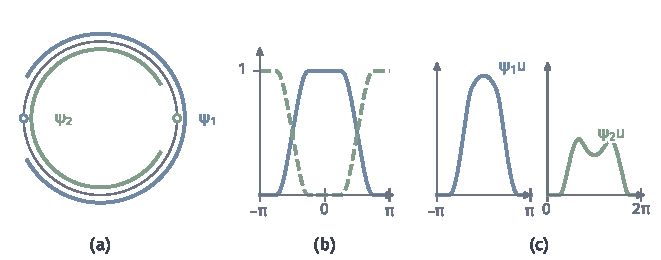
\includegraphics[width=112mm]{figures/04-spaces-measures-and-geometry/04-manifolds/matplotlib/mcalc-chart-cover/figure.pdf}
  \caption{圆周上的有限覆盖与单位分解。(a)两张角度图，分别漏掉$(-1,0)$与$(1,0)$（空心圆），蓝弧与绿弧是$\psi_1,\psi_2$的支撑，每个支撑严格落在所在的图内。(b)$\psi_1$（实线）与$\psi_2=1-\psi_1$（虚线），横轴是角度$\theta$。(c)$u=1+\tfrac12\cos\theta$被切成的两段$\psi_1u$与$\psi_2u$，分别画在各自的图中，都是区间上紧支撑的函数。}
  \label{fig:mcalc-chart-cover}
\end{BookInlineFigure}

在每个$\overline{U_\alpha}$上，度量矩阵的特征值有正的上下界，所以$\lVert\xi\rVert_g$与坐标欧氏长度$\lVert\xi\rVert_2$、$\mathrm dV_g$与$\mathrm d\bm x$在常数倍内可比。单位分解函数及其导数有界，并且乘积规则对弱梯度仍成立：
\[
\operatorname{grad}(\psi_\alpha u)=\psi_\alpha\operatorname{grad}u+u\operatorname{grad}\psi_\alpha .
\]

由这些估计可以得到$\lVert\cdot\rVert'$与$\lVert\cdot\rVert_{W^{1,p}}$等价，并且换用另一组有限覆盖或单位分解只改变等价常数。完整写出常数需要把上面的上下界逐项收集，篇幅较长；结论的含义是，一阶Sobolev空间作为函数集合只取决于光滑结构，度量与覆盖的选择只影响范数的数值。

这一等价性是搬运欧氏结论的通道。例如光滑函数的稠密性：对$u\in W^{1,p}(M)$，把每个$(\psi_\alpha u)\circ\varphi_\alpha^{-1}$用第~\ref{chap:smoothing-weak-derivatives}章的磨光逼近，再拉回求和，得到逼近$u$的光滑函数。磨光后支撑仍落在稍大的坐标域内，这正是要求$\overline{U_\alpha}$落在更大坐标图中的原因。

高阶空间$W^{k,p}(M)$可以同样用坐标图定义，也可以用协变导数$\nabla^ku$内在地定义，两者在紧流形上等价，证明需要逐阶比较协变导数与坐标偏导数，读者可查阅几何分析方面的教材。第~\ref{chap:sobolev-spaces}章的连续嵌入与紧嵌入也可以经有限覆盖搬到紧流形上，所得常数依赖覆盖与度量。

\paragraph{带边界的情形}
紧的带边界流形上，边界附近的坐标图取值于半空间。第~\ref{chap:sobolev-spaces}章在半空间或光滑边界区域上建立的延拓、迹与约束子空间，经边界坐标图搬到流形上，须逐项核对两件事。

一是所用的欧氏结论是否要求边界光滑：流形的边界在定义上光滑，但带角点的区域不在这一框架内。二是结论在坐标变换下是否保持：例如“迹为零”的子空间与坐标无关，而迹的具体范数依赖坐标与度量。Dirichlet条件对应$W^{1,p}$中“迹为零”的闭子空间，Neumann条件则不进入空间的定义，而是在弱形式中由边界项自然体现。

\paragraph{非紧流形}
非紧流形上，有限覆盖不复存在，逐图的控制与整体范数有限是两回事。$\mathbb R$上的常函数$u\equiv1$在每个有界坐标区间上都属于$L^p$与$W^{1,p}$，整体上却不属于$L^p(\mathbb R)$。为区分这两层，记$L^p_{\mathrm{loc}}$与$W^{1,p}_{\mathrm{loc}}$为在每个紧子集上满足相应条件的函数。局部空间不依赖度量，整体空间则依赖度量。

整体空间对度量的依赖在非紧时不再是范数等价那么简单。$\mathbb R$上取$g=\mathrm dx^2$与$g'=(1+x^2)^2\mathrm dx^2$，二者的体积密度之比为$1+x^2$，无界。函数$u(x)=(1+\lvert x\rvert)^{-1}$满足
\[
\int_{\mathbb R}u^2\,\mathrm dx<\infty,\qquad\int_{\mathbb R}u^2(1+x^2)\,\mathrm dx=\infty ,
\]
第二个积分发散是因为被积函数在无穷远处趋于$1$。所以$u\in L^2(\mathbb R,g)$却$u\notin L^2(\mathbb R,g')$，两个空间是不同的集合。

欧氏结论也不能无条件继承。紧流形上$W^{1,2}(M)\hookrightarrow L^2(M)$是紧嵌入；$\mathbb R$上则不然。取支撑含于$(0,1)$的非零光滑函数$\varphi$及其平移$\varphi(x-k)$，$k=1,2,\ldots$，它们在$W^{1,2}(\mathbb R)$中有界，而由于支撑不交，
\[
\lVert\varphi(\cdot-k)-\varphi(\cdot-l)\rVert_{L^2}=\sqrt2\,\lVert\varphi\rVert_{L^2},\qquad k\neq l ,
\]
所以这列函数没有$L^2$收敛的子列。这与第~\ref{chap:functions-as-vectors}章中无限维闭球不紧的现象同源：平移把一个固定的函数送到互不相交的位置，相当于在$L^2$中给出无穷多个互相正交的方向。

非紧流形上嵌入不等式的常数还可能因体积或曲率失去一致的控制而失效，使用时须先核对流形的整体几何条件。
